% Options for packages loaded elsewhere
\PassOptionsToPackage{unicode}{hyperref}
\PassOptionsToPackage{hyphens}{url}
%
\documentclass[
]{article}
\usepackage{amsmath,amssymb}
\usepackage{lmodern}
\usepackage{iftex}
\ifPDFTeX
  \usepackage[T1]{fontenc}
  \usepackage[utf8]{inputenc}
  \usepackage{textcomp} % provide euro and other symbols
\else % if luatex or xetex
  \usepackage{unicode-math}
  \defaultfontfeatures{Scale=MatchLowercase}
  \defaultfontfeatures[\rmfamily]{Ligatures=TeX,Scale=1}
\fi
% Use upquote if available, for straight quotes in verbatim environments
\IfFileExists{upquote.sty}{\usepackage{upquote}}{}
\IfFileExists{microtype.sty}{% use microtype if available
  \usepackage[]{microtype}
  \UseMicrotypeSet[protrusion]{basicmath} % disable protrusion for tt fonts
}{}
\makeatletter
\@ifundefined{KOMAClassName}{% if non-KOMA class
  \IfFileExists{parskip.sty}{%
    \usepackage{parskip}
  }{% else
    \setlength{\parindent}{0pt}
    \setlength{\parskip}{6pt plus 2pt minus 1pt}}
}{% if KOMA class
  \KOMAoptions{parskip=half}}
\makeatother
\usepackage{xcolor}
\usepackage[margin=1in]{geometry}
\usepackage{graphicx}
\makeatletter
\def\maxwidth{\ifdim\Gin@nat@width>\linewidth\linewidth\else\Gin@nat@width\fi}
\def\maxheight{\ifdim\Gin@nat@height>\textheight\textheight\else\Gin@nat@height\fi}
\makeatother
% Scale images if necessary, so that they will not overflow the page
% margins by default, and it is still possible to overwrite the defaults
% using explicit options in \includegraphics[width, height, ...]{}
\setkeys{Gin}{width=\maxwidth,height=\maxheight,keepaspectratio}
% Set default figure placement to htbp
\makeatletter
\def\fps@figure{htbp}
\makeatother
\setlength{\emergencystretch}{3em} % prevent overfull lines
\providecommand{\tightlist}{%
  \setlength{\itemsep}{0pt}\setlength{\parskip}{0pt}}
\setcounter{secnumdepth}{-\maxdimen} % remove section numbering
\ifLuaTeX
  \usepackage{selnolig}  % disable illegal ligatures
\fi
\IfFileExists{bookmark.sty}{\usepackage{bookmark}}{\usepackage{hyperref}}
\IfFileExists{xurl.sty}{\usepackage{xurl}}{} % add URL line breaks if available
\urlstyle{same} % disable monospaced font for URLs
\hypersetup{
  pdftitle={Topic 1. Introduction to Environmental Data Analysis},
  pdfauthor={ENS-215},
  hidelinks,
  pdfcreator={LaTeX via pandoc}}

\title{Topic 1. Introduction to \emph{Environmental Data Analysis}}
\author{ENS-215}
\date{Winter 2025}

\begin{document}
\maketitle

{
\setcounter{tocdepth}{2}
\tableofcontents
}
\hypertarget{why-learn-data-science}{%
\subsection{Why learn data science?}\label{why-learn-data-science}}

\begin{quote}
\emph{It is pretty clear that almost every field today needs data-savvy
researchers. It has become something as basic as driving a car in our
intellectual work}\\
-- Saul Perlmutter (2011 Nobel Laureate in Physics)
\end{quote}

Data science is a rapidly growing field and is becoming an integral part
of nearly all fields of study, including the Earth and environmental
sciences. In the past few years, programs specifically focused on data
analytics for Earth and environmental sciences have been created or
expanded at many prominent institutions (Stanford, Berkeley,U. Chicago,
and UC Boulder to name a few).

The demand in the academic, public, and private sectors for
environmental scientists with skills is data analytics has been growing
and job and research opportunities are strong. The articles below
provide a nice overview on the rising importance of data science in the
environmental fields.

\begin{itemize}
\item
  \url{https://eos.org/opinions/training-the-next-generation-of-physical-data-scientists}
\item
  \url{https://earth.stanford.edu/news/21st-century-earth-science-computer-intensive-and-data-driven}
\item
  \url{https://www.earthdatascience.org/blog/earth-data-scientist-demand/}
\item
  \textbf{Why learn programming?}

  \begin{itemize}
  \tightlist
  \item
    Allows you to analyze, model, and interpret data that is often
    impossible (or exceedingly difficult) to do otherwise
  \item
    Streamlines your workflow, allowing you to conduct analysis in a
    documented, reproducible, and efficient manner
  \item
    Opens the door to answering a whole new set of questions in your
    research
  \item
    Highly marketable skill set in science/engineering careers as well
    as non-science careers
  \end{itemize}
\item
  \textbf{Why learn R?}

  \begin{itemize}
  \tightlist
  \item
    One of the most popular programming languages for data analysis and
    statistics
  \item
    User friendly with lots of available support material and large user
    community
  \item
    Tens of thousands of packages available to facilitate a wide range
    of analytical and visualization tasks
  \item
    Allows for efficient and automated access to thousands of
    databases/datasets across the environmental and geosciences (as well
    as across many other fields)\\
  \item
    Widely used by many leading environmental and geoscience
    organization, with widespread usage at the USGS
  \item
    Highly desired programming language when applying for jobs and grad
    school\\
  \item
    You can create cool figures, maps, and visualizations
  \end{itemize}

  \begin{figure}
  \centering
  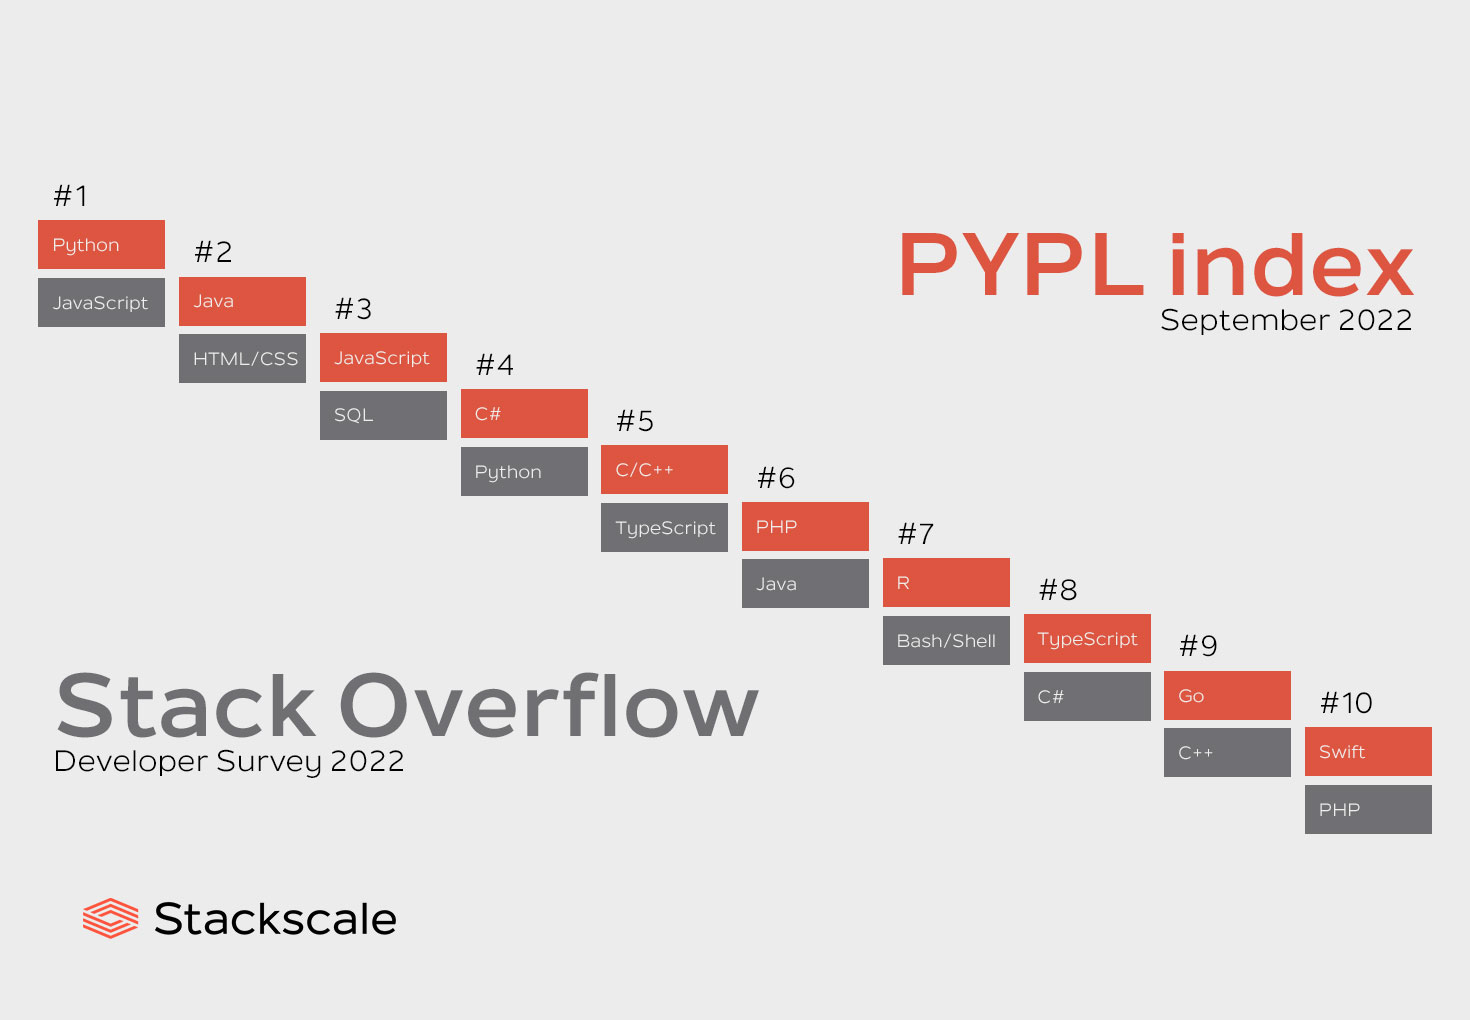
\includegraphics{http://stahlm.github.io/ENS_215/Winter_2025/Images/popular-programming-languages-ranking-2022.jpg}
  \caption{\textbf{R is rapidly growing in popularity}\\
  source
  (\url{https://www.stackscale.com/blog/most-popular-programming-languages})}
  \end{figure}
\end{itemize}

~

\hypertarget{interactive-figures-are-easy-to-make}{%
\paragraph{\texorpdfstring{\textbf{Interactive figures are easy to
make}}{Interactive figures are easy to make}}\label{interactive-figures-are-easy-to-make}}

\hypertarget{programming-in-r}{%
\subsection{Programming in R}\label{programming-in-r}}

\hypertarget{rstudio-ide}{%
\subsubsection{RStudio IDE}\label{rstudio-ide}}

We will write and run our code within the RStudio Integrated Development
Environment (IDE). RStudio allows us to write, excute (run), and debug
code, along with view output and plots, within a single integrated
environment.

\hypertarget{getting-help-in-r}{%
\subsubsection{Getting help in R}\label{getting-help-in-r}}

There are lots of resources for
\href{https://stahlm.github.io/ENS_215/Winter_2025/Syllabus.html\#useful_linksresources}{getting
help in R}. In addition to me and your classmates, there is a massive
amount of help available freely online (a quick Google search typically
yields an answer to just about any R question). There are also many
websites devoted to teaching R.

Visit Union College's very own \href{https://muse.union.edu/cda/}{Center
for Data Analytics}! It is located in \textbf{Wold 010} and hosts a data
science help desk, where expert students and faculty who staff the help
desk can help answer your questions. The Center for Data Analytics also
host regular training workshops and guest speakers.

You can also get help directly in R Studio by typing
\texttt{?term\_of\_interest\_here} in the R \textbf{Console} or by
searching in the \textbf{Help} bar on the right-hand side of your
RStudio window.

Your textbooks \href{https://r4ds.hadley.nz/}{\emph{R for Data Science}}
and \href{https://moderndive.com/v2/index.html}{\emph{ModernDive}} are
also amazing resources and freely available online in a nice searchable
format.

\href{https://posit.co/resources/cheatsheets/}{R Cheatsheets} are also
amazing resources that succinctly summarize many different aspects of R.
I will hand these out throughout the term, though you can find them
freely available here.

\hypertarget{syllabus-and-course-logistics}{%
\subsection{Syllabus and course
logistics}\label{syllabus-and-course-logistics}}

\begin{itemize}
\tightlist
\item
  \textbf{Course logistics}

  \begin{itemize}
  \tightlist
  \item
    You will find all course related materials (e.g.~schedule/syllabus,
    assignments, notes, course policies,\ldots) at our
    \href{https://stahlm.github.io/ENS_215/Winter_2025/Home.html}{class
    webpage}
  \item
    Assignments will be submitted through Nexus. You MUST use the
    specified naming convention for the files you submit.
  \item
    Attendance and on-time arrival is critical and your grade will be
    affected by unexcused absences and late arrivals! You will quickly
    fall behind if you miss class or arrive late.
  \item
    We will use computers during class and lab, however you should ONLY
    use your computer for class related activities. This means that you
    should close unrelated material prior to the start of class and that
    your should not check email, news, Instagram, Twitter,\ldots{}
    during class.
  \item
    Carefully read the syllabus. It has important information about
    grading, course policies, and tips for success in the class.
  \item
    In each class we will work through code examples in R. I will post
    my R Notebooks (which act as lecture notes/slides) to the course
    website. DO NOT simply copy and paste the code from these notebooks.
    You will not learn the material by doing this. You should type out
    the code, think carefully about what it means, run the code, and
    examine the output before moving on to the next step.
  \item
    Get a binder to hold class notes/handouts. This binder will act as a
    course specific textbook.
  \item
    You need to be an active learner in this class. Learning programming
    and data analysis cannot be done passively.\\
  \item
    You should recognize that there will be challenges and bumps as you
    are learning how to code. You are not alone in this (everyone even
    experienced programmers hit roadblocks when they work). There are
    TONS of resources out there to help you. A quick Google search of
    whatever problem you've hit or something new that you'd like to see
    an example for, will almost always yield tons of information
    directly related to your question.
  \end{itemize}
\end{itemize}

\end{document}
